\documentclass[border=8pt]{standalone}
\usepackage[utf8]{inputenc}
\usepackage{tikz}
\tikzset{
  debole/.style = {rectangle, draw, thick, fill=blue!8, double, double distance=1.5pt, minimum width=26mm, minimum height=16mm, font=\small},
  attr/.style   = {circle, draw, thick, fill=white, minimum size=5pt, inner sep=0},
  pk/.style     = {circle, draw, thick, fill=black, minimum size=5pt, inner sep=0},
  link/.style   = {thick}, et/.style = {font=\footnotesize}
}
\begin{document}
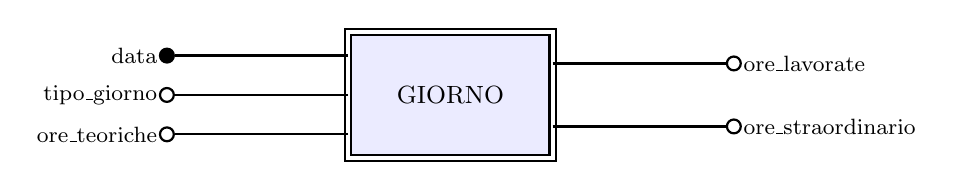
\begin{tikzpicture}
  \node[debole] (E) {GIORNO};
  \node[pk]   (d)  at (-3.6, 0.5){}; \draw[link] (-1.3, 0.5)--(d);  \node[et,left] at (d)  {data};
  \node[attr] (tg) at (-3.6, 0.0){}; \draw[link] (-1.3, 0.0)--(tg); \node[et,left] at (tg) {tipo\_giorno};
  \node[attr] (ot) at (-3.6,-0.5){}; \draw[link] (-1.3,-0.5)--(ot); \node[et,left] at (ot) {ore\_teoriche};
  \node[attr] (ol) at ( 3.6, 0.4){}; \draw[link] ( 1.3, 0.4)--(ol); \node[et,right] at (ol) {ore\_lavorate};
  \node[attr] (os) at ( 3.6,-0.4){}; \draw[link] ( 1.3,-0.4)--(os); \node[et,right] at (os) {ore\_straordinario};
\end{tikzpicture}
\end{document}
